\documentclass[svgnames,sigplan,10pt]{acmart}

\usepackage{times}
\usepackage{fullpage}

\usepackage{graphicx}
\usepackage{amssymb}
\usepackage{algorithm}
\usepackage[noend]{distribalgo}
\usepackage{fixme}
\usepackage{alltt}
\usepackage{xspace}
\usepackage{adjustbox}
\usepackage{caption}
\usepackage{subcaption}

\newcommand{\ex}{$\mathcal{E}$}
\newcommand{\pp}{$\mathcal{P}$}
\newcommand{\ppm}{\mathcal{P}}
\newcommand{\pqm}{\mathcal{Q}}
\newcommand{\oom}{\mathcal{O}}
\newcommand{\oo}{$\mathcal{O}$}
\newcommand{\cc}{$\mathcal{C}$}
\newcommand{\ccm}{\mathcal{C}}
\newcommand{\kk}{$\mathcal{K}$}
\newcommand{\vv}{$\mathcal{V}$}
\newcommand{\vvm}{\mathcal{V}}
\newcommand{\vvt}{$\mathcal{V}$}
\newcommand{\rr}{$\mathcal{R}$}
\newcommand{\rrm}{\mathcal{R}}
\newcommand{\sst}{$\mathcal{S}$}
\newcommand{\ssm}{\mathcal{S}}
\newcommand{\ip}{\mathcal{I}}
%
% S-SMR
\newcommand{\ssmr}{\mbox{S-SMR}\xspace}
\newcommand{\ssmrshort}{Scalable SMR}
\newcommand{\ssmrlong}{Scalable State Machine Replication}
%
% DS-SMR
\newcommand{\dssmr}{\mbox{DS-SMR}}
\newcommand{\dssmrshort}{Dynamic S-SMR}
\newcommand{\dssmrlong}{Dynamic Scalable State Machine Replication}
%
% The new DS-SMR system
\newcommand{\dynastar}{\mbox{DynaStar}\xspace}

\newcommand{\libname}{DynaStar} 
\newcommand{\appname}{Chirper}
%
\newcommand{\rmcast}{r-mcast}
\newcommand{\rmdel}{r-deliver}
\newcommand{\amcast}{a-mcast}
\newcommand{\amdel}{a-deliver}
\newcommand{\parts}{partition}
\newcommand{\coloralgo}{Yellow}

\newcommand{\mynote}[3]{
   \fbox{\bfseries\sffamily\scriptsize#1}
   {\small$\blacktriangleright$\textsf{\emph{\color{#3}{#2}}}$\blacktriangleleft$}}
\newcommand{\fp}[1]{\mynote{Fernando}{#1}{Red}}
\newcommand{\eb}[1]{\mynote{Eduardo}{#1}{Green}}
\newcommand{\ef}[1]{\mynote{Enrique}{#1}{Blue}}
\newcommand{\lle}[1]{\mynote{Long}{#1}{Cerulean}}
\newcommand{\rjs}[1]{\mynote{Robert}{#1}{Gold}}

\newcommand{\red}[1]{\textit{\textcolor{red}{#1}}}

% do not change these values
\baselineskip 12pt
\textheight 9in
\textwidth 6.5in
\oddsidemargin 0in
\topmargin 0in
\headheight 0in
\headsep 0in

\begin{document}

\title{\dynastar: Optimized Dynamic Partitioning for\\ Scalable State Machine Replication}
\author{Long Hoang Le$^1$, Enrique Fynn$^1$, Mojtaba Eslahi-Kelorazi$^1$, Robert Soul\'{e}$^1$ and Fernando Pedone$^1$ \\
\small {\em  $^1$Universit\`{a} della Svizzera italiana (USI), Switzerland} \\ [2mm]
\small Submission type: Research (12 pages, excluding references)
}
\date{}
\maketitle

% \thispagestyle{empty}

\begin{abstract}
  
Sharding and replication are the mechanisms of choice of most scalable and fault-tolerant distributed systems.
The performance of a sharded system, however, heavily depends on the partitioning of the data: in order to scale, most commands must involve a single shard and load must be balanced across shards.
Estimating a good partitioning of the application state is challenging since it requires a priori information about the workload.
Moreover, even if such information is available, access patterns may change during system execution.
A good partitioning of the data for uniform access patterns may lead to poor performance under skewed access patterns.
The paper introduces DynaStar, a scalable and fault-tolerant system that supports dynamic state partitioning.
This means that DynaStar does not require a priori knowledge about the workload and can seamlessly adapt to workload variations.
The paper describes DynaStar design and implementation, and presents a detailed performance evaluation using two benchmarks, a social network based on real data and TPC-C.


\end{abstract}

%!TEX root =  main.tex
\section{Introduction}


\begin{figure*}[ht!]
  \centering
  \begin{subfigure}[b]{0.45\textwidth}
    \centering
    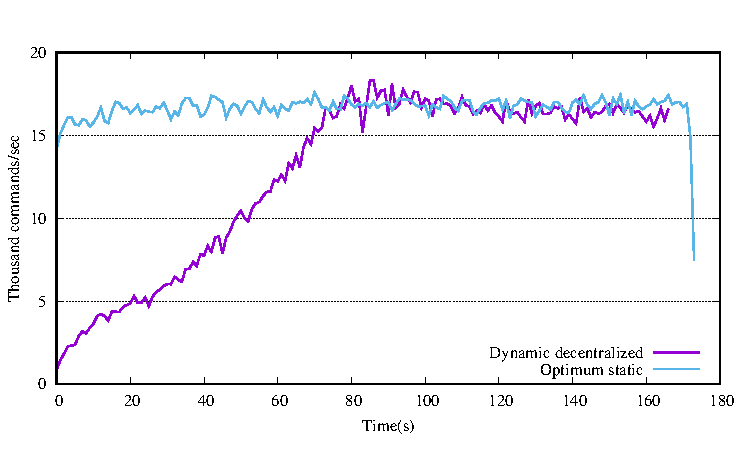
\includegraphics[width=0.95\columnwidth]{figures/motivation-tp-strong-locality}    
  \label{fig:motivation}
    \caption{Throughput with strong locality.}
  \end{subfigure}
  \begin{subfigure}[b]{0.45\textwidth}
    \centering
    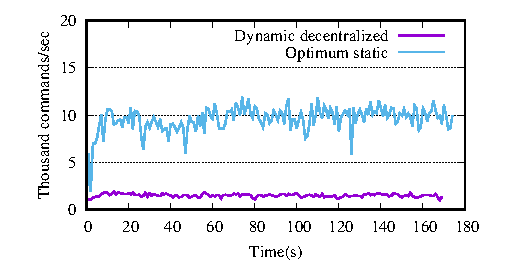
\includegraphics[width=0.95\columnwidth]{figures/motivation-tp-weak-locality}
    \caption{Throughput with weak locality}
  \end{subfigure} \\
  \begin{subfigure}[b]{0.45\textwidth}
    \centering
    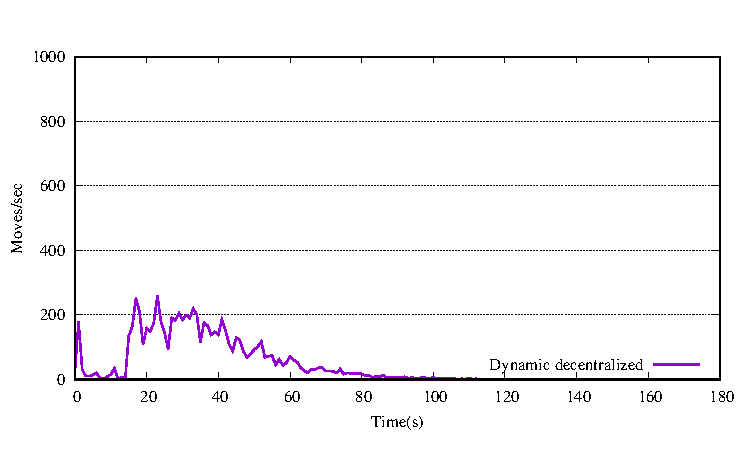
\includegraphics[width=0.95\columnwidth]{figures/motivation-moves-strong-locality}
    \caption{Number of move commands with strong locality.}
  \end{subfigure}
  \begin{subfigure}[b]{0.45\textwidth}
    \centering
    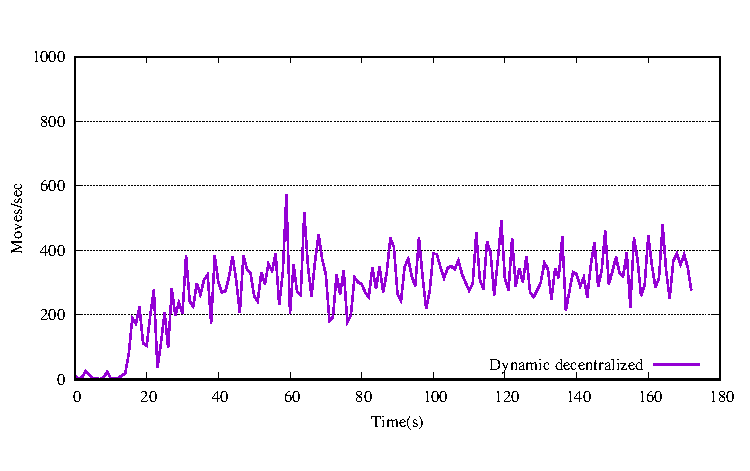
\includegraphics[width=0.95\columnwidth]{figures/motivation-moves-weak-locality}
    \caption{Number of move commands with weak locality}
  \end{subfigure} 
\end{figure*}




State machine replication (SMR) is a fundamental technique for
building fault-tolerant systems and services. With SMR, state is
replicated on a set of servers and each replica deterministically
executes the same sequence of client commands in order to maintain
consistency~\cite{Lam78,Sch90}. Unfortunately, classic state machine replication does not
scale, since each replica must execute every command. In order to
improve the scalability of SMR, several systems have investigated the
use of state partitioning~(e.g., \cite{corbett2013spanner, bezerra2014ssmr,Glendenning:2011kj,
  Aguilera:2007,bli16edcc}).

In principle, increasing the number of partitions should result in
increased system performance. However, if executing a command
requires that the system access multiple partitions, then performance
can actually decrease, due to overhead from ordering and coordinating commands across partitions to
ensure strong consistency. Moreover, if data is not distributed
carefully, then load imbalances can nullify the benefits of
partitioning.  Thus, an ideal partitioning scheme is one that would
both (i) allow commands to be executed at a single partition only, and (ii) evenly distribute data so that load is balanced among partitions.
We refer to workloads that can be
partitioned in a way that satisfies these two properties as exhibiting
\emph{strong locality}.

Broadly speaking, there are two classes of techniques for
partitioning: \emph{static} and \emph{dynamic}.
Figure~\ref{fig:motivation} shows the result of a motivating experiment
that highlights the shortcomings of both of these approaches. In
the experiment, we show the throughput and number of state moves
over time with two different workloads; one with strong locality
and one with weak locality. For brevity, we postpone the details
of the experimental setup until Section~\ref{sec:experiments}.

Static schemes choose an immutable assignment of objects to partitions in
advance.  A prominent example of a
static scheme is S-SMR~\cite{bezerra2014ssmr}. One problem with static schemes is
that they cannot adapt as workloads change over time (e.g., in social
networks users join and leave the system, connections are created and
removed). One could imagine a static scheme that re-partitioned the
data based on every change in workload, \fp{this seems to contradict the notion of static}but such a scheme would be
impossible to implement, since it would require a priori knowledge of
the workload. Figure~\ref{fig:motivation} shows the theoretical
optimal throughput one could achieve with a ``perfect'' static scheme.


Dynamic schemes are designed to address the problem with static
schemes.  Dynamic schemes assume no prior knowledge of the workload,
and move data to partitions on-demand in order to avoid
multi-partition commands. A prominent example of a dynamic scheme is
DS-SMR~\cite{hoang2016}. Unfortunately, existing dynamic schemes assume
workloads with strong locality. \fp{apparently not true in general, that's how ds-smr works}As Figure~\ref{fig:motivation} shows,
for workloads with weak-locality, DS-SMR suffers from instability due
to constantly moving data from one partition to another.


In this paper, we introduce \dynastar, a new approach to the state
partitioning problem designed to address these challenges.  \dynastar
is \emph{dynamic}. It does not require any a priori knowledge about
the workload, and it adapts to workload changes on-the-fly. However,
it is able to achieve throughputs comparable to the unrealizable
perfect static scheme. The key idea behind \dynastar is that it
minimizes the number of state relocations by monitoring the workload,
and re-computing an optimal partitioning on demand using a static
partitioner, we chose to use METIS partitioning algorithm~\cite{Abou-Rjeili:2006}
as an example of a static partitioner.
%ef.: Changed so we allow plug-and-play partitioners
\fp{we should probably say that it preserves consistency}

With \dynastar, a location oracle maintains two data structures: (i) a
mapping of objects to partitions, and (ii) a \emph{workload graph}
with objects as vertices and edges as commands that access the
objects.  When a client submits a command, it must first contact the
location oracle to discover the partitions on which the objects are
stored.  If the command accesses objects in multiple partitions, the
oracle issues a move command to the partitions, re-locating objects to
a single partition. Of course, when re-locating an object, the oracle
is faced with a choice of which partition to use as a destination.
\dynastar chooses the optimal partition for relocation (i.e., one that
would minimize the number of state relocations) by partitioning the
workload graph using the METIS partitioner.




We have fully implemented \dynastar and compared its performance to
the dynamic partitioning protocol proposed by Long et
al.~\cite{hoang2016} and to the optimized static partitioning scheme.
Our prototype can handle workload graphs with half a million variables
and tens of millions of connections.  In workloads that present strong
locality, all three protocols eventually delivered comparable
performance, although \dynastar converged more quickly than the
decentralized scheme.  In workloads with weak locality, however,
\dynastar \emph{outperformed both} schemes.  The reason for the
surprisingly high performance of \dynastar compared to the optimized
static partitioning scheme is that \textbf{we need to explain this!!!
:-)} \ef{If the cost of migrating the object outperforms the cost of 
signaling partitions, why performance get similar when we have more partitions?} 
\lle{in static scheme, partitions exchange signal in every global commands,
while, in dynamic scheme, there is chance that partitions already have
data, thus no communication needed. More over, signaling is a two-way mechanism,
while moving objects in dynamic scheme is only one-way, which leads to less data
is being exchanged}

The paper makes the following contributions:
\begin{itemize}
\item It introduces \dynastar and discusses its implementation. 
\item It evaluates different partitioning schemes for state machine replication under a variety of conditions.
\item It describes \appname{} to demonstrate how \libname{} can be used to implement a scalable social network service.
\item It presents a detailed experimental evaluation of \dynastar including real social network graphs with half a million users and 14 million edges.
\end{itemize}

The rest of the paper is structured as follows.
Section~\ref{sec:sysmodel} describes our system model.
Section~\ref{sec:background} reviews existing scalable state machine replication approaches.
Section~\ref{sec:dssmr} introduces \dssmr{}; we explain the technique in detail and argue about its correctness.
Section~\ref{sec:implementation} details the implementation of \libname\ and \appname{}.
Section~\ref{sec:experiments} reports on the results of our experiments with \dssmr{}.
Section~\ref{sec:rw} surveys related work and
Section~\ref{sec:conclusion} concludes the paper.




%% %% Because single-partition commands are much more efficient than
%% %% multi-partition commands (i.e., in some cases by a factor of more than
%% %% 10x), the performance of a distributed storage system is particularly sensitive to the way
%% %% the service state is partitioned.


%% \subsection{State Machine Replication}

%% State machine replication (SMR) is a well-established technique to
%% develop highly available services (e.g.,
%% \cite{Shvachko:2003,Ghemawat:2003,Burrows:2006,MacCormick:2004}).  In
%% essence, the idea is that replicas deterministically execute the same
%% sequence of client commands in the same order and in doing so traverse
%% the same sequence of states and produce the same results.  State
%% machine replication provides configurable fault tolerance in the sense
%% that the system can be set to tolerate any number of faulty replicas.
%% Increasing the number of replicas, however, will not scale performance
%% since each replica must execute every command.  Unfortunately,
%% increasing the number of replicas will not scale performance since
%% each replica must execute every command.

%% S-SMR relies on an atomic multicast primitive to consistently order
%% commands within and across partitions.  Commands that access objects
%% located in a single partition (i.e., single-partition commands) are
%% multicast to the concerned partition and executed like in classical
%% SMR.  Commands that access objects located in multiple partitions
%% (i.e., multi-partition commands) are multicast to all involved
%% partitions.  To prevent command interleaves that violate strong
%% consistency, partitions coordinate during the execution of
%% multi-partition commands.



%% \subsection{Motivating Example}

%!TEX root =  main.tex
\section{System model and definitions}
\label{sec:sysmodel}

In this section, we present the system model, and define our
correctness criterion (i.e., linearizability). Additionally, because
\dynastar relies on two variations of a multicast primitive for
communication, we discuss them below. When the protocol requires that
commands be consistently ordered across partitions, \dynastar uses
atomic multicast. Otherwise, it uses a reliable multicast, which has
less overhead.


%\red{How do we use reliable multicast, as opposed to atomic?}
%\red{Do we need this primitive? Or is it just inherited from the artifact?}
%\lle{Partitions (and oracle) in \dynastar use reliable multicast to exchange
% objects and signals }
%% S-SMR relies on an atomic multicast primitive to consistently order
%% commands within and across partitions.  Commands that access objects
%% located in a single partition (i.e., single-partition commands) are
%% multicast to the concerned partition and executed like in classical
%% SMR.  Commands that access objects located in multiple partitions
%% (i.e., multi-partition commands) are multicast to all involved
%% partitions.  To prevent command interleaves that violate strong
%% consistency, partitions coordinate during the execution of
%% multi-partition commands.




\subsection{Processes and communication}

We consider a distributed system consisting of an unbounded set of
client processes $\ccm = \{c_1, c_2, ...\}$ and a bounded set of
server processes (replicas) $\ssm = \{s_1, ..., s_n\}$.  Set $\ssm$ is
divided into disjoint groups of servers $\ssm_0, ..., \ssm_k$.
Processes are either \emph{correct}, if they never fail, or
\emph{faulty}, otherwise.  In either case, processes do not experience
arbitrary behavior (i.e., no Byzantine failures).

Processes communicate by message passing, using either one-to-one or
one-to-many communication.  The system is asynchronous: there is no
bound on message delay or on relative process speed.  One-to-one
communication uses primitives $send(p,m)$ and $receive(m)$, where $m$
is a message and $p$ is the process $m$ is addressed to.  If sender
and receiver are correct, then every message sent is eventually
received.
%
One-to-many communication relies on reliable multicast and atomic
multicast,\footnote{Solving atomic multicast requires additional
  assumptions~\cite{CT96,FLP85}. In the following, we simply assume
  the existence of an atomic multicast oracle.}  defined in
sections~\ref{sec:rmcast} and \ref{sec:amcast}, respectively.


\subsection{Correctness criterion}
\label{sec:correctcrit}

Our consistency criterion is linearizability.  A system is
\emph{linearizable} if there is a way to reorder the client commands
in a sequence that (i)~respects the semantics of the commands, as
defined in their sequential specifications, and (ii)~respects the
real-time precedence of commands~\cite{Attiya04}.


\subsection{Reliable multicast}
\label{sec:rmcast}

To reliably multicast a message $m$ to a set of groups $\gamma$,
processes use primitive \rmcast$(\gamma, m)$.  Message $m$ is
delivered at the destinations with \rmdel$(m)$.  Reliable multicast
has the following properties:

\begin{itemize}

    \item[--] If a correct process \rmcast{}s $m$, then every correct
      process in $\gamma$ \rmdel{}s $m$ \emph{(validity)}.
    
    \item[--] If a correct process \rmdel{}s $m$, then every correct
      process in $\gamma$ \rmdel{}s $m$ \emph{(agreement)}.
    
    \item[--] For any message $m$, every process $p$ in $\gamma$
      \rmdel{}s $m$ at most once, and only if some process has
      \rmcast{} $m$ to $\gamma$ previously \emph{(integrity)}.
    
\end{itemize}

\subsection{Atomic multicast}
\label{sec:amcast}

To atomically multicast a message $m$ to a set of groups $\gamma$,
processes use primitive \amcast$(\gamma, m)$.  Message $m$ is
delivered at the destinations with \amdel$(m)$.  We define delivery
order $<$ as follows: $m < m'$ iff there exists a process that
delivers $m$ before $m'$.

Atomic multicast ensures the following properties:

\begin{itemize}
    
    \item[--] If a correct process \amcast{}s $m$, every correct
      process in a group in $\gamma$ \amdel{}s $m$ \emph{(validity)}.
    
    \item[--] If a process \amdel{}s $m$, then every correct process
      in a group in $\gamma$ \amdel{}s $m$ \emph{(uniform agreement)}.
    
    \item[--] For any message $m$, every process \amdel{}s $m$ at most
      once, and only if some process has \amcast{} $m$ previously
      \emph{(integrity)}.
    
    \item[--] The delivery order is acyclic \emph{(atomic order)}.

    \item[--] For any messages $m$ and $m'$ and any processes $p$ and
      $q$ such that $p \in g$, $q \in h$ and $\{ g, h \} \subseteq
      \gamma$, if $p$ delivers $m$ and $q$ delivers $m'$, then either
      $p$ delivers $m'$ before $m$ or $q$ delivers $m$ before $m'$
      \emph{(prefix order)}.
    
\end{itemize}

Atomic broadcast is a special case of atomic multicast in which there
is a single group of processes.


%!TEX root =  main.tex
\section{Background}
\label{sec:background}


\dynastar builds on
prior work on scalable state machine replication
~\cite{bezerra2014ssmr,hoang2016}, which in turn, builds on classic
state machine replication. In this section, we briefly review these
techniques. 

\subsection{State machine replication}
\label{sec:smr}

State machine replication is a fundamental approach to implementing fault-tolerant services by replicating servers, and coordinating the execution of client commands at replicas~\cite{Lam78,Sch90}. 
Every replica has a full copy of the service state, identified by a set of state variables $\vvm = \{v_1, ..., v_m\}$.
A command is a sequence of deterministic operations that can read and modify the state.

%SMR ensures linearizability by coordinating the execution of commands in the replicas: 
%Replicas execute commands submitted by the clients in the same order. 
By starting in the same initial state and executing the same sequence of deterministic commands in the same order, servers make the same state changes and produce the same reply for each command. 
To guarantee that servers deliver the same sequence of commands, SMR can be implemented with atomic broadcast: commands are atomically broadcast to all servers, and all correct servers deliver and execute the same sequence of commands \cite{BJ87b,DSU04}.

Despite its simple execution model, classical SMR does not scale: adding resources (e.g., replicas) will not translate into sustainable improvements in throughput. 
%This happens for two reasons. 
%First, the underlying communication protocol needed to ensure ordered message delivery may itself not scale (i.e., a communication bottleneck). 
%Second, every command must be executed sequentially by each replica (i.e., an execution bottleneck).
%
Several approaches have been proposed to address SMR's scalability limitations. 
In the following, we review two state machine replication approaches that partition the service's state and replicate each partition (e.g., \cite{Glendenning:2011kj,hoang2016,Marandi:2011dj}).
%Scalable State Machine Replication (\ssmr), an approach that partitions the service's state and replicates each partition (e.g., \cite{Glendenning:2011kj,Marandi:2011dj,hoang2016}).


\subsection{Static state partitioning (S-SMR)}
%\subsection{Scalable State Machine Replication (S-SMR)}
%\subsection{Scalable replication with static state partitioning}
%\subsection{S-SMR with static partitioning}
\label{sec:ssmr}

In S-SMR~\cite{bezerra2014ssmr}, the service state \vvt\ is composed of $k$ partitions, $\ppm_1, ..., \ppm_k$, where each partition $\ppm_i$ is statically assigned to server group $\ssm_i$. 
For brevity, we say that server $s$ belongs to $\ppm_i$ meaning that $s \in \ssm_i$, and say ``multicast to $\ppm_i$" meaning ``multicast to server group $\ssm_i$".
S-SMR relies on a \emph{static oracle}, which tells clients which partitions are accessed by each command.
%\footnote{The oracle returns a set with the partitions accessed by the command, but this set does not need to be minimal; it may contain all partitions in the worst case, when the partitions accessed by the command cannot be determined before the command is executed.}

To execute a command, a client multicasts the command to the appropriate partitions, as determined by the oracle.
Commands that access a single partition are executed as in classical SMR: replicas of the concerned partition agree on the execution order and each replica executes the command independently.
In the case of a multi-partition command, replicas of the involved partitions deliver the command and then may need to exchange state, since some partitions may not have all the values read in the command.
This mechanism allows commands to execute seamlessly despite the partitioned state.

%\begin{algorithm}[t!]
\small

\begin{distribalgo}[1]

\vspace{1mm}

\INDENT{\emph{Initialization:}}
    \STATE $\forall C \in \mathcal{K} : rcvd\_signals(C) \leftarrow \emptyset$
    \STATE $\forall C \in \mathcal{K} : rcvd\_variables(C) \leftarrow \emptyset$
\ENDINDENT

\vspace{1.25mm}
\INDENT{\emph{Command $C$ is submitted by a client as follows:}}
    \STATE $C.dests \leftarrow oracle(C)$ \label{algline:oracle} 
	\STATE \amcast$(C.dests, C)$ \label{algline:climcast}
	\STATE wait for reply
\ENDINDENT

\vspace{1.25mm}
\INDENT{\emph{Server $s$ of partition \pp\ executes command $C$ as follows:}}
	\INDENT{\textbf{when} \amdel$(C)$}
	    \STATE $others \leftarrow C.dests \setminus \{\ppm{}\}$
	    \STATE \rmcast$(others, signal(C))$ \label{algline:mcastsignals}
		\FOR{each operation $op$ in $C$}
			\IF{$op$ is $read(v)$}
			    \IF{$v \in \ppm$}
			        \STATE \rmcast$(others, \langle v, C.id \rangle)$ \label{algline:multicastv}
			    \ELSE
			        \STATE \textbf{wait until} $v \in rcvd\_variables(C)$ \label{algline:waitvariable}
			        \STATE update $v$ with the value in $rcvd\_variables(C)$
			    \ENDIF
			\ENDIF
			\STATE execute $op$ \label{algline:executeopck}
		\ENDFOR
		\STATE \textbf{wait until} $rcvd\_signals(C) = others$ \label{algline:waitsignals}
		\STATE send reply to client \label{algline:sendreply}
	\ENDINDENT
	
	\vspace{1.25mm}
	\INDENT{\textbf{when} \rmdel$(signal(C))$ from partition $\ppm'$}
	    \STATE $rcvd\_signals(C) \leftarrow rcvd\_signals(C) \cup \{\ppm'\}$
	\ENDINDENT

	\vspace{1.25mm}
	\INDENT{\textbf{when} \rmdel$(\langle v, C.id \rangle)$}
	    \STATE $rcvd\_variables(C) \leftarrow rcvd\_variables(C) \cup \{v\}$
	\ENDINDENT
			
\ENDINDENT

\vspace{1.7mm}

\textbf{Algorithm variables:}

\vspace{1.25mm}

$\mathcal{K}$: the set of all possible commands

\vspace{1mm}

$C.id$: unique identifier of command $C$

\vspace{1mm}

$oracle(C)$: function that returns a superset of the partitions accessed by $C$

\vspace{1mm}

$C.dests$: set of partitions to which $C$ is multicast

\vspace{1mm}

$others$: set of all partitions, other than \pp{}, where $C$ is executed.

\vspace{1mm}

$signal(C)$: signal exchanged to ensure linearizability

\vspace{1mm}

$rcvd\_signals(C)$: set of all partitions that already signaled \pp\ regarding $C$

\vspace{1mm}

$rcvd\_variables(C)$: set of all variables received from other partitions in order to execute $C$

\caption{Scalable State Machine Replication (\ssmr)}
\label{alg:ssmr}
\end{distribalgo}
\end{algorithm}

%\begin{figure*}
%\begin{minipage}[b]{1\linewidth} % A minipage that covers the whole width of the page
%\centering
%      \includegraphics[width=1.0\linewidth]{figures/move_case_1}
%\end{minipage}
%\caption{Consulting the oracle and issuing a command are done in multiple calls to \amcast{}. White boxes represent actions of the client proxy.}
%\label{fig:move_case_1}
%\end{figure*}

%Algorithm~\ref{alg:ssmr} shows precisely how S-SMR operates. 
In more detail, when a server $s$ of partition $\ppm$, while executing a command $C$, needs to read variable $v$, there are two possibilities:
either $v$ belongs to the local partition $\ppm$,
or it is part of a remote partition $\ppm'$. 
If $v$ is local, $s$ will retrieve its value and send it to the servers of other partitions concerned by $C$;
if $v$ is remote, $s$ will wait until its value is received from a server of $\ppm'$. 
A write operation on $v$ does not depend on the previous value of $v$, not requiring communication between partitions, even if $v$ is not assigned to the partition of the server executing $C$.
To ensure linearizability, all partitions involved in the execution of a multi-partition command $C$ must coordinate before a reply can be sent to the client.
%To understand why, consider the non-linearizable execution shown in Figure~\ref{fig:whysignals}~(a).
%This execution is not linearizable because the only equivalent sequential execution requires $C_y$ to precede $C_{xy}$ and $C_{xy}$ to precede $C_x$, thus $C_y$ would precede $C_x$.
%Although this execution does not violate atomic order, it contradicts real-time ordering, in which $C_x$ precedes $C_y$.
In \ssmr{}, partitions exchange signals while executing multi-partition commands~\cite{bezerra2014ssmr}.
This guarantees linearizability, at the cost of synchronizing partitions.

S-SMR improves on classical SMR by allowing single-partition commands to scale. 
Multi-partition commands, however, have limited performance. 
One way to reduce the number of multi-partition commands is to dynamically put variables that are usually accessed together in the same partition.
Unfortunately, \ssmr 's static mapping of variables to partitions does not allow the service to dynamically adapt to different access patterns.

%\subsection{S-SMR with dynamic partitioning}
%\subsection{Scalable replication with decentralized dynamic state partitioning}
%\subsection{Dynamic decentralized state partitioning}
\subsection{Dynamic state partitioning (DS-SMR)}

\dssmr{}~\cite{hoang2016} defines a dynamic mapping of variables to partitions.
Each variable $v$ is mapped to a partition $\ppm$, that is, $v \in \ppm$.
Such a mapping is managed by the partitioning oracle, which, differently from \ssmr, is now implemented as a replicated service run by a group of server processes.
The oracle allows the mapping of variables to partitions to be retrieved or changed during execution.
In more detail, \dssmr\ distinguishes five types of commands:
$access(\omega)$ is an application command that accesses (reads or writes) variables in set $\omega \subseteq \vvm$,
$create(v)$ creates a new variable $v$ and initially maps it to a partition defined by the oracle,
$delete(v)$ removes $v$ from the service state,
% resulting in $part(v) = \emptyset$,
$move(v,\ppm_s,\ppm_d)$ moves variable $v$ from partition $\ppm_s$ to partition $\ppm_d$,
and $consult(C)$ asks the oracle which variables are accessed by command $C$, and which partition contains each of them.
The reply from the oracle is called a $prophecy$, and usually consists of a set of tuples $\langle v, \ppm \rangle$, meaning $v \in \ppm$.
% The other possible values for a prophecy are $ok$ and $nok$, which mean that command can and cannot be executed, respectively (more details in Section~\ref{sec:algorithm}).
%If $v$ is not part of the service state (i.e., it was deleted or never created), the prophecy will contain~$\langle v, \emptyset \rangle$.

% explain which partitions deliver each partitioning command:
% how are access, consult, create, move and delete implemented?

%Once the oracle is in place, 
Clients consult the oracle to know which partitions each command should be multicast to, based on the objects accessed by the command.
If the reply received from the oracle tells the client that the command accesses a single partition, the client multicasts the command to that partition.
If the command accesses objects from multiple partitions, the client first multicasts one or more $move$ commands to the oracle and to the involved partitions, with the intent of having all variables in the same partition.
Then, the command itself is multicast to the one partition that now holds all variables accessed by the command.
If a subsequent command accesses the same variables, it will also access a single partition.
Thus, the access patterns of commands will shape the mapping of variables to partitions, reducing the number of multi-partition commands.

Consulting the oracle and issuing the application command are done with separate calls to atomic multicast in \dssmr{}.
It may happen that, between those operations, the partitioning changes.
%We illustrate this in Figure~\ref{fig:move_case_1}.
%Commands $C_1$ and $C_2$ read variable $x$.
%Since partitioning is dynamic, the client issuing the commands first consults the oracle before multicasting each command.
%$C_1$ executes without the interference of other commands, so consulting the oracle and multicasting the command only once is enough for $C_1$ to be executed.
%However, before $C_2$ is multicast to $\ppm_1$, another client issues a $move$ command that relocates $x$ to $\ppm_2$.
%When $C_2$ is delivered at the servers of $\ppm_1$, the command is not executed, since $x$ is not available at $\ppm_1$ anymore.
%A similar situation may arise when a command accesses variables from multiple partitions, as it consists of multicasting at least three commands separately: $consult$, $move$ and $access$.
%The partitioning can change between the execution of any two of those commands.
%\begin{figure}[b!]
%  \includegraphics[width=\linewidth]{figures/move_case_1}
%  \caption{Consulting the oracle and issuing an application command consist of multiple calls to \amcast{}.}
%  \label{fig:move_case_1}
%\end{figure}
% \pagebreak
To solve this problem, the client multicasts the set of variables accessed along with each access command.
Upon delivery, each server checks the set of variables sent by the client.
If all variables in the set belong to the local partition, the command is executed; otherwise, a $retry$ message is sent back to the client.
When the client receives a $retry$ message, it consults the oracle again, possibly moves variables across partitions, and then reissues the access command.
To guarantee termination, if the command fails a certain number of times, the client multicasts the command to all partitions and the servers execute it as in the original \ssmr{}.


%!TEX root =  main.tex
\section{State partitioning with \dynastar}
%\section{Optimized dynamic state partitioning with \dynastar}
\label{sec:dynastar}

In this section, we overview \dynastar's key ideas, present the protocol in detail, discuss some performance optimizations, and argue about \dynastar's correctness.

\subsection{Overview}
%\subsection{State partitioning as a graph problem}

%\dynastar improves DS-SMR to cope with workloads that exhibit both strong and weak locality.
%In the presence of strong locality, \dynastar converges more quickly than the decentralized dynamic scheme.
%Under weak locality (i.e., workloads that cannot be perfectly partitioned), \dynastar largely outperforms DS-SMR.

The key insights of \dynastar are to create the workload graph on-the-fly and use graph partitioning techniques to efficiently relocate application state on-demand.
\begin{itemize}
\item \emph{On-the-fly workload modeling.}
\dynastar models a service workload as a graph $G = (V, E)$, where vertices represent state variables and edges dependencies between variables.
An edge connects two variables in the graph if a command accesses both of them.
A location oracle builds the workload graph based on feedback from the clients or partitions, as commands are executed.
\item \emph{On-demand relocation of service state.}
Periodically, the oracle computes a partitioning of the workload graph and multicasts to the partitions.
Based on this partitioning and the current location of variables, the partitions determine the destination for commands that access variables spread over multiple partitions.
Variables are moved on demand to the destination partition where the command will be executed. After the execution, variables are moved back to the source partition to keep the optimized partitioning.
\end{itemize}

In \dynastar a move request is multicast together with the command that triggered the request.
%a partition executes a command right after it has gathered all variables it needs.
Therefore, differently from DS-SMR, \dynastar ensures termination without resorting to expensive mechanisms (i.e., S-SMR).


\subsection{The \dynastar protocol}

Algorithms~\ref{alg:client_proxy}, \ref{alg:server_proxy}, and \ref{alg:oracle_proxy} describe the client, server and oracle processes, respectively. 
For brevity, we omit the delete command since the coordination involved in the create and delete commands are analogous. 
In the discussion in this section, every command involves the oracle.
The oracle is replicated and handled as a partition.
In the next section, we explain how clients can use a cache to avoid the oracle in the execution of most commands.


\subsubsection{The client process} 

To execute a command, the client atomically multicasts the command to the oracle (Algorithm 1).
The oracle replies with a prophecy, which may already tell the client that the command cannot be executed (e.g., it needs a variable that does not exist, it tries to create a variable that already exists).
If the command can be executed, the client receives a prophecy containing the partition where the command will be executed. The client then waits for the result of the execution of the command.


% The client must retry the command if the partition cannot execute the command.
% This happens if the cache on client is invalid, some of the variables needed by the command were moved to another partition due a new partitioning. 
%To ensure that a command is eventually executed, after retrying a few times, the client falls back to using \ssmr{}, multicasting the command to all partitions (and the oracle, in case of a create or delete command).

\subsubsection{The server process} 

All servers keep a workload graph in their memory. When a server delivers a command $C$, multicast by the oracle, it first checks if it has all variables needed by the command. If the server has all such variables, it executes the command and sends the response back to the client (Tasks 1a and 3 in Algorithm~\ref{alg:server_proxy}).
If not all the variables needed by the command are in that partition, the server issues a move command that involves all partitions containing the needed variables (Task 1b and 2).
%If one or more variables are not stored in a single partition, the server returns a message to the client to retry the operation.
%This happens if the oracle moved some variables to another partition as part of another command. 
In this case, a server in the source partitions reliably multicasts all the needed variables stored locally to the destination partition and waits to receive them back.
Destination partition waits for a message from each source partition. Once all variables needed are available, destination partition executes the command $C$, sends the response back to the client, and returns the variables to their source.
Periodically, the servers deliver a new partitioning plan from the oracle (Task 4). Each server will send the variables to the designated partition as in the plan and wait for variables from other partitions. Once a server receives all variables, it updates its location map accordingly.
%When a server delivers a message to create a variable (and similarly to delete an existing variable), it coordinates with the oracle (Task 3).
%The exchange of signals between the partition where the variable will be created and the oracle ensures that interleaved executions between create and delete commands will not lead to violations of linearizability (i.e., this is essentially the execution of a multi-partition command involving the oracle and a partition~\cite{bezerra2014ssmr}).
To determine the destination partition for a command, the servers uses the last computed partitioning.

\subsubsection{The oracle} 

When the oracle delivers a request, it distinguishes between two cases (Task 1 in Algorithm~\ref{alg:oracle_proxy}).
\begin{itemize}
\item If the command is to create a variable $v$, and $v$ does not already exist, the oracle chooses a random partition for $v$, multicasts the create command to the partition and itself, and returns the partition to the client as a prophecy (Figure~\ref{fig:oracle_repartition}).
\item If the command reads and writes existing variables, the oracle first checks that all such variables exist.
If the variables exist and they are all in a single partition, the oracle multicasts the command to that partition for execution.
If the variables are distributed in multiple partitions, the oracle determines the destination partition, and atomically multicasts a command to the involved partitions and to itself so that all variables are gathered at the destination partition.
The destination partition executes the command once it has received all variables needed by the command, then returns those variables to their source partition.

%In either case, oracle returns a prophecy back to the client with the destination partition.
\end{itemize}

\begin{algorithm}[h!]
\small

\begin{distribalgo}[1]

%\vspace{1.0mm}

\INDENT{\colorbox{\coloralgo}{To issue a command $C$, the client does:}}

\vspace{1.0mm}
	\STATE \amcast$($oracle, $exec(C))$
%	\COMMENT{$C$ could be either $create(v)$ or $access(\omega)$}
	\STATE wait for $prophecy$
	\IF[if receive $nok$ then...]{$prophecy = nok$}
		\STATE $reply \leftarrow prophecy$
		\COMMENT{...there's nothing to execute}
	\ELSE[in this case, $prophecy$ is $(dest)$]
		\STATE wait for $reponse$ from a server in $prophecy$
		\STATE $reply \leftarrow reponse$
	\ENDIF
\STATE return $reply$ to the application
\ENDINDENT

\caption{Client}
\label{alg:client_proxy}
\end{distribalgo}
\end{algorithm}
\begin{algorithm}[h!]
\small

\begin{distribalgo}[1]

\vspace{1.0mm}

\INDENT{To execute a command $C$, the server proxy in partition $P$ does:}

    \vspace{1.0mm}
    
    \INDENT{\textbf{when} \rmdel$( \langle val, C \rangle )$}
        \STATE $rcvd\_msgs \leftarrow rcvd\_msgs \cup \{\langle val, C \rangle\}$
    \ENDINDENT

    \vspace{1.0mm}

    \INDENT{\textbf{when} \amdel$(C)$}

    \vspace{1.0mm}

        \IF{\underline{$C$ is an $access$ command}}
            \IF{$\exists v \in C.vars : v \not\in P$}
                \STATE reply with $retry$
            \ELSE
                \STATE have the command executed by the application server
                \STATE send the reply to the client
            \ENDIF
        

        \vspace{1.0mm}
    
        \ELSIF{\underline{$C$ is a $move(v,P_d)$ command}}
            \IF{$P \neq P_d$}
                \IF{$v \in P$}
                    \STATE \rmcast$(P_d$,$\langle v, C \rangle)$
                    \STATE $P \leftarrow P \setminus \{v\}$
                \ELSE
                    \STATE \rmcast$(P_d$,$\langle null, C \rangle)$
                \ENDIF
            \ELSE
                \STATE wait until $\exists val : \langle val, C \rangle \in rcvd\_msgs$
                \IF{$val \neq null$}
                    \STATE $v \leftarrow val$
                    \STATE $P \leftarrow P \cup \{v\}$
                \ENDIF
            \ENDIF
        
        \vspace{1.0mm}
    
        \ELSIF{\underline{$C$ is a $create(v)$ command}}
            \STATE wait until $\langle val, C \rangle \in rcvd\_msgs$
            \IF{$val = ok$}
                \STATE $P \leftarrow P \cup \{v\}$
%                \STATE reply with $success$
%            \ELSE
%                \STATE reply with $retry$
            \ENDIF
        
        \vspace{1.0mm}
        
        \ELSIF{\underline{$C$ is a $delete(v)$ command}}
            \IF{$v \in P$}
                \STATE $P \leftarrow P \setminus \{v\}$
%                \STATE reply with $success$
%            \ELSE
%                \STATE reply with $retry$
            \ENDIF
        \ENDIF
    \ENDINDENT
\ENDINDENT

\caption{\dssmr\ Server Proxy}
\label{alg:server_proxy}
\end{distribalgo}
\end{algorithm}
\begin{algorithm}[t!]
\small

\begin{distribalgo}[1]

%\vspace{1.0mm}

	\INDENT{\colorbox{\coloralgo}{\textbf{when} \amdel$(consult(C))$}}
%		\INDENT{\textbf{case} $C$ is a $consult(C_c)$ command:}
%			\STATE $update(G_W, \omega)$
			\INDENT{\textbf{case} $C$ is an $access(\omega)$ command:}
				\IF[if $v$ doesn't exist:]{$\exists v \in \omega : \parts(\{v\}) = \bot$}
					\STATE $prophecy \leftarrow nok$
					\COMMENT{tell the client}
				\ELSE[if all vars in $\omega$ exist]
%					\STATE $dests \leftarrow \emptyset$
%					\FOR{each $v \in \omega$}
%						\STATE $dests \leftarrow dests \cup partition(v)$
%					\ENDFOR
					\STATE $dests \leftarrow \parts(\omega)$
					\COMMENT{get all partition involved}
					\IF[if only one partition:]{$|dests| = 1$}
						\STATE $prophecy \leftarrow (dests,\emptyset)$
						\COMMENT{tell client which partition}
					\ELSE[if multiple partitions involved]
						\STATE $\ppm_d \leftarrow target(G_W, \omega)$
						\COMMENT{$\ppm_d$ will store all vars in $\omega$}
						\FOR[for each involved var $v$]{each $v \in \omega$}
							\STATE $\ppm_s \leftarrow \parts(\{v\})$
							\COMMENT{$\ppm_s$ is $v$'s current partition}
							\IF[if $v$ not in $\ppm_d$:]{$\ppm_s \neq \ppm_d$}
								\STATE $aux \leftarrow \{oracle,\ppm_s,\ppm_d\}$
								\COMMENT{move $v$ from $\ppm_s$...}
								\STATE \amcast$(aux$, $move(v,\ppm_s,\ppm_d))$
								\COMMENT{...to $\ppm_d$}
							\ENDIF 
						\ENDFOR
						\STATE $prophecy \leftarrow (\{\ppm_d\},dests\ \cup \{oracle\})$
					\ENDIF 
				\ENDIF
			\ENDINDENT
			\INDENT{\textbf{case} $C$ is a $create(v)$ command:}
				\IF[if $v$ already exists...]{$\parts(\{v\}) \neq \bot$}
					\STATE $prophecy \leftarrow nok$
					\COMMENT{...notify client}
				\ELSE[if $v$ doesn't exist...]
					\STATE $\ppm \leftarrow target(G_W, \{v\})$
					\COMMENT{...determine $v$'s partition and}
					\STATE $prophecy \leftarrow (\{ \ppm, oracle \}, \emptyset)$
					\COMMENT{prepare client's response}
				\ENDIF
			\ENDINDENT
			\STATE send $prophecy$ to the client
%			\INDENT{\textbf{case} $C_c$ is a $delete(v)$ command:}
%				\IF{$partition(v) = \bot$}
%					\STATE $prophecy \leftarrow ok$
%				\ELSE
%					\STATE $prophecy \leftarrow (\{ \ppm : v \in \ppm, oracle \}, -)$
%				\ENDIF
%			\ENDINDENT
%		\ENDINDENT
	\ENDINDENT
	\vspace{1.0mm}

	\INDENT{\colorbox{\coloralgo}{\textbf{when} \amdel$(move(v,\ppm_s,\ppm_d))$}}
%        \INDENT{\textbf{case} $C$ is a $move(v,\ppm_s,\ppm_d)$ command:}
                \STATE $\ppm_s \leftarrow \ppm_s \setminus \{v\}$
                \COMMENT{update $v$'s current and...}
                \STATE $\ppm_d \leftarrow \ppm_d \cup      \{v\}$
                \COMMENT{...new partition}
                \STATE send $ok$ to the client
	\ENDINDENT

        \vspace{1.0mm}
    
	\INDENT{\colorbox{\coloralgo}{\textbf{when} \amdel$(create(v))$}}
%	\INDENT{\textbf{case} $C$ is a $create(v)$ command:}
		\STATE let $\ppm_c \in C.dests \setminus \{oracle\}$
		\COMMENT{var created in $\ppm_c$}
		\STATE \rmcast$(\ppm_c, \langle signal, C \rangle )$
		\COMMENT{exchange signal to...}
		\STATE wait until $\langle signal, C \rangle \in rcvd\_msgs$
		\COMMENT{...coordinate partitions}
		\STATE $\ppm_c \leftarrow \ppm_c \cup      \{v\}$
                \STATE send $ok$ to the client
	\ENDINDENT

	\vspace{1.0mm}
	\INDENT{\colorbox{\coloralgo}{\textbf{when} \rmdel$( \langle val, C \rangle )$}}
		\STATE $rcvd\_msgs \leftarrow rcvd\_msgs \cup \{\langle val, C \rangle\}$
	\ENDINDENT
	
	\vspace{1.0mm}
	\INDENT{\colorbox{\coloralgo}{\textbf{function} \parts$(vars)$}}
		\STATE $aux \leftarrow \{ \ppm : \exists v \in vars \cap \ppm \}$
		\STATE return $aux$
	\ENDINDENT
	
%	\vspace{1.0mm}
	\rule{83mm}{0.4pt}
%	\vspace{0.1mm}

	\INDENT{\colorbox{\coloralgo}{\textbf{when} \amdel$(hint(V_h,E_h))$}}
		\STATE update $G_W$ with $(V_h,E_h)$
		\STATE send $ok$ to the client
	\ENDINDENT
	
	\vspace{1.0mm}
    
	\INDENT{\colorbox{\coloralgo}{\textbf{periodically do}}}
		\STATE compute ideal partition $\ip_1, ..., \ip_m$ from $G_W$
	\ENDINDENT
	
	\vspace{1.0mm}
    
	\INDENT{\colorbox{\coloralgo}{\textbf{function} target$(vars)$}}
		\STATE $\ppm \leftarrow$ compute target from $vars$ and $\ppm_1, ..., \ppm_m$
		\STATE return $\ppm$
	\ENDINDENT	
	
%	\vspace{1.0mm}
%        
%	\INDENT{\textbf{case} $C$ is a $delete(v)$ command:}
%		\STATE let $\ppm_d$ be $\ppm : \{\ppm\} = C.dests \setminus \{$oracle$\}$
%		\STATE $\ppm_c \leftarrow \ppm_c \setminus      \{v\}$
%		\STATE \rmcast$(\ppm_c, \langle ok, C \rangle )$
%			\STATE wait until $\exists val : \langle val, C \rangle \in rcvd\_msgs$
%	\ENDINDENT

%\ENDINDENT

\caption{Oracle}
\label{alg:oracle_proxy}
\end{distribalgo}
\end{algorithm}

\begin{figure*}
\begin{minipage}[b]{1\linewidth} % A minipage that covers the whole width of the page
\centering
      \includegraphics[width=0.9\linewidth]{figures/dynastar}
\end{minipage}
\caption{The execution of a create command and a write command in \dynastar.}
\label{fig:oracle_repartition}
\end{figure*}

Upon delivering a create (Task 2), the oracle updates its partition information.
As part of a create command, the oracle coordinates with the partition to ensure correctness (Task 3)~\cite{bezerra2014ssmr}.
%
The oracle also keeps track of the workload graph by receiving hints with variables (i.e., vertices in the graph) and executing commands (i.e., edges in the graph). These hints can be submitted by the clients or by the partitions, which collect data upon executing commands and periodically inform the oracle (Task 4).
The oracle computes a partitioning plan of the graph and multicasts it to all servers and to itself. Upon delivering new partition plan, the oracle updates its location map accordingly (Task 5).
% The oracle also keeps track of the workload graph, computes a partitioning of the graph, and determines the destination partition for move operations.
% To maintain the workload graph (Task 5), the oracle receives hints with variables (i.e., vertices in the graph) and executed commands (i.e., edges in the graph).

To compute an optimized partitioning, the oracle uses a graph partitioner.
A new partitioning can be requested by the application, by a partition, or by the oracle itself (e.g., upon delivering a certain number of hints).
To determine the destination partition of a set of variables, as part of a move, the oracle uses 
% the current location of variables and 
the last computed partitioning.

\subsection{Performance optimizations}
%\subsection{Performance optimizations}
\label{sec:optm}

\textbf{Caching.} In the algorithm presented in the previous section, clients always need to involve the oracle, and the oracle dispatches every command to the partitions for execution.
Obviously, if every command involves the oracle, the system is unlikely to scale, as the oracle will likely become a bottleneck.
To address this issue, clients are equipped with a location cache.
Before submitting a command to the oracle, the client checks its location cache.
If the cache contains the partition of the variables needed by the command and all variables are in a single destination partition, the client can atomically multicast the command to the partition and avoid contacting the oracle. 

The client still needs to contact the oracle in one of these situations:
%(a)~according to client's cache, not all variables accessed by the command are in the same partition and it is necessary to move variables;
%(b)~the cache contains outdated information, and the command is multicast to a partition that does not contain all needed variables; or
(a)~the cache contains outdated information; or
(b)~the command is a create, in which it must involve the oracle, as explained before.
%If the cache contains outdated information and the addressed partition does not contain all the variables accessed by the command, the partition tells the client to retry the command.
If the cache contains outdated information and the addressed partition does not have the information of all the variables accessed by the command, the partition tells the client to retry the command.
In this case, the client contacts the oracle and then updates its cache with the oracle's response.

\textbf{Subgraph on servers}. If all partitions have to keep a copy of the the workload graph, scaling is also a problem as the graph is growing over time. Thus, servers only keep a subgraph of variables they are holding and the neighbors of those objects, by observing the access pattern of the commands. Using this subgraph only, the servers can compute the destination partition for executing commands without the need of having the full graph.

%!TEX root =  main.tex
\clearpage
\subsection{Correctness}
\label{sec:correctness}

In this section, we argue that \dynastar is safe (i.e., it ensures linearizability) and live (i.e., it ensures termination).

To prove that \dynastar ensures linearizability, we must show that for any execution $\sigma$ of the system, there is a total order $\pi$ on client commands that 
(i)~respects the semantics of the commands, as defined in their sequential specifications, and 
(ii)~respects the real-time precedence of commands~(Section~\ref{sec:correctcrit}).
%
Let $\pi$ be a total order of operations in $\sigma$ that respects $<$, the order atomic multicast induces on commands.

To argue that $\pi$ respects the semantics of  commands, let $C_i$ be the $i$-th command in $\pi$ and $p$ a process in partition $\ppm_p$ that executes $C_i$.
%Let $C_i$ be the $i$-th command in $\pi$ and $p$ a process in partition $\ppm_p$ that executes $C_i$.
We claim that when $p$ executes $C_i$, it has updated values of variables in $vars(C_i)$, the variables accessed by $C_i$.
We proof the claim by induction on $i$.
The base step trivially holds from the fact that variables are initialized correctly.
Let $v \in vars(C_i)$, $C_v$ be the last client command before $C_i$ in $\pi$ that accesses $v$, and $q$ a process in $\ppm_q$ that executes $C_v$.
From the inductive hypothesis, $q$ has an updated value of $v$ when it executes $C_v$.
There are two cases to consider:
(a)~$p = q$. In this case, $p$ obviously has an updated value of $v$ when it executes $C_i$ since no other command accesses $v$ between $C_v$ and $C_i$.
(b)~$p \neq q$. 
Since processes in the same partition execute the same commands, it must be that $\ppm_p \neq \ppm_q$.
From the algorithm, when $q$ executes $C_v$, $v \in \ppm_q$ and when $p$ executes $C_i$, $v \in \ppm_p$.
Thus, $q$ executed a command to move $v$ to another partition after executing $C_v$ and $p$ executed a command to move $v$ to $\ppm_p$ before executing $C_i$.
Since there is no command that accesses $v$ between $C_v$ and $C_i$ in $\pi$, $q$ has an updated $v$ when it executes $C_v$ (from inductive hypothesis), and $p$ receives the value of $v$ at $q$, it follows that $p$ has an updated $v$ when it executes $C_i$.

% DISCLAIMER: in the proof below, I assumed a single process per partition. While I'm pretty sure it works for multiple processes per partition, in some future refinement this should be added to the proof. Also see related picture showing cases (a) and (b) below. Perhaps we should include such a picture too in a future version.
%
We now argue that there is a total order $\pi$ that respects the real-time precedence of commands in $\sigma$.
Assume $C_i$ ends before $C_j$ starts, or more precisely, the time $C_i$ ends at a client is smaller than the time $C_j$ starts at a client, $tec(C_i) < tsc(C_j)$.
Since the time $C_i$ ends at the server from which the client receives the response for $C_i$ is smaller than the time $C_i$ ends at the client, $tes(C_i) < tec(C_i)$, and the time $C_j$ starts at the client is smaller than the time $C_j$ starts at the first server, $tsc(C_j) < tss(C_j)$, we conclude that $tes(C_i) < tss(C_j)$.

We must show that either $C_i < C_j$; or neither $C_i < C_j$ nor $C_j < C_i$.
For a contradiction, assume that $C_j < ... < Z_k < ... < C_i$, where $Z_k$ is a client or a move command.
Let $Z_k$ be delivered by partition $\ppm_k$.
There are two cases: 
\begin{enumerate}
\item[(a)] $Z_{k+1}$ is a client command delivered by partition $\ppm_k$.
In this case, since $Z_{k+1}$ only starts after $Z_k$ at a server, it follows that $tes(Z_k) < tss(Z_{k+1})$.
\item[(b)] $Z_{k+1}$ is a move command that involves $\ppm_k$ as source and $\ppm_{k+1}$ as destination.
At $\ppm_k$, $tes(Z_k) < tss(Z_{k+1})$ since the move is only executed after $Z_k$.
Since servers in $\ppm_k$ must send one or more variables to servers in $\ppm_{k+1}$, it must be that $tss(Z_{k+1}) < tes(Z_{k+1})$.
Thus, it follows that $tes(Z_{k+1}) < tss(Z_{k+2})$.
\end{enumerate}
From the two cases above, we conclude that $tes(C_j) < tss(C_i)$, a contradiction.
Therefore, either $C_i < C_j$ and from the definition of $\pi$, $C_i$ precedes $C_j$ or neither $C_i < C_j$ nor $C_j < C_i$, and there is a total order in which $C_i$ precedes $C_j$.
%\begin{figure}
%\centering
%\includegraphics[width=1.2\linewidth,angle=-90]{figures/IMG_7203.JPG}
%\caption{Two cases in proof.}
%\end{figure}

For termination, we argue that every correct client eventually receives a reply different than $retry$ for every command $C$ that it issues.
This assumes that every partition (including the oracle partition) is always operational, despite the failure of some servers in the partition.
For a contradiction, assume that some client submits a command $C$ that always returns $retry$.
Therefore, from the algorithm, whenever $C$ is delivered at a partition, the partition does not contain all the variables needed by $C$.
As a consequence, the client eventually falls back to \ssmr\ and multicasts $C$ to all partitions and $C$ is executed as a multi-partition command, which is guaranteed to succeed, a contradiction that concludes our argument.








%!TEX root =  ssmr_ieee.tex
\section{Implementation}
\label{sec:implementation}

In this section, we describe Eyrie, a library that implements S-SMR, and Volery, a service that provides Zookeeper's API.
Volery can be configured to provide high availability by means of state-machine replication and to use Eyrie to combine high availability and throughput scalability.
Volery was built with Eyrie, combining high availability and throughput scalability (by means of scalable state-machine replication).
Both Eyrie and Volery were implemented in Java.
%In this section, we detail the implementation of Eyrie, a library that implements Scalable State-Machine Replication (Section \ref{sec:libjssmr}) and present Volery, an application that provides the Zookeeper API (Section \ref{sec:zkssmr}).
%%Volery can be configured to provide high availability by means of state-machine replication and to use Eyrie to combine high availability and throughput scalability.
%Volery was built with Eyrie, combining high availability and throughput scalability (by means of scalable state-machine replication).
%Both Eyrie and Volery were implemented in Java.

%, Section \ref{sec:zkssmr}) and Chirper (a Twitter-like application, Section \ref{sec:chirper}).
% There are two main aspects of it to consider: (i) how it handles communication between partitions to ensure linearizability and (ii) how transparent it is for developers to migrate an existing fully-replicated service to Scalable SMR.

\subsection{Eyrie}
\label{sec:libjssmr}

One of the main goals of Eyrie is to make the implementation of services based on Scalable SMR as easy as possible. 
To use Eyrie, the user (i.e., service designer) must extend two classes, \verb#PRObject# and \verb#StateMachine#. 
%Even though they are simple to implement, their implementation is required by Eyrie. 
Class \verb#PartitioningOracle# has a default implementation, but the user is encouraged to override its methods. 
%Finally, the user must provide a configuration file describing the partitions and the atomic multicast protocol to be used.



\subsubsection{The \texttt{PRObject} class}

Eyrie supports partial replication (i.e., some objects may be replicated in some partitions, not all). 
Therefore, when executing a command, a replica might not have local access to some of the objects involved in the execution of the command. 
%
%The user informs Eyrie which object classes are partially replicated by extending the \verb#PRObject# class.
The user informs to Eyrie which object classes are partially replicated by extending the \verb#PRObject# class. Each object of such class may be stored locally or remotely, but the application code is agnostic to that. All calls to methods of such objects are intercepted by Eyrie, transparently to the user.

%Eyrie uses AspectJ\footnote{http://eclipse.org/aspectj} to intercept method calls for all subclasses of \verb#PRObject#, which correspond to remote objects. 
%Internally, the aspect related to such remote method invocations communicates with the user's subclass of \verb#StateMachine# in order \fixme{Too vague; what's done really?}to find out what is the command being executed at the moment \ul{and make sure that the execution is linearizable.}

Eyrie uses AspectJ\footnote{http://eclipse.org/aspectj} to intercept method calls for all subclasses of \verb#PRObject#. 
Internally, the aspect related to such method invocations communicates with the \verb#StateMachine# instance in order to (i) determine if the object is stored locally or remotely and (ii) ensure that the object is up-to-date when each command is executed.

Each replica has a local copy of all \verb#PRObject# objects. 
When a remote object is received, replicas in the local partition $P_L$ must update their local copy of the object with an up-to-date value. 
For this purpose, the user must provide implementations for the methods \verb#getDiff(Partition p)# and \verb#updateFromDiff(Object diff)#. The former is used by the remote partition $P_R$, which owns the object, to calculate a delta between the old value currently held by $P_L$ and the newest value, held by $P_R$. Such implementations may be as simple as returning the full object, which is then serialized and, upon deserialization in $P_L$, completely overwrites the old copy of the object. However, it also allows the user to implement caching mechanisms. Since \verb#getDiff# takes a partition as parameter, the user may keep track of what was the last value received by $P_L$, and then return a (possibly small) diff, instead of the whole object, which is then applied to the object with the user-provided method \verb#updateFromDiff#.

%The \verb#PRObject# class also contains several methods that are used internally by Eyrie. For instance, it contains an index of all PRObjects in the system, along with their corresponding partitions. By having such knowledge, each object knows where its up-to-date copy is, so that they can always have recent up-to-date values.

To avoid unnecessary communication, the user may optionally mark some methods of their \verb#PRObject# subclasses as local, by annotating them with \verb#@LocalMethodCall#. Calls to such methods are not intercepted by the library, sparing communication when the user sees fit. Although the command that contains a call to such a method still has to be delivered and executed by all partitions that hold objects accessed by the command, that particular local method does not require an up-to-date object. For example, say a command $C$ accesses objects $O_1$ and $O_2$, respectively, in partitions $P_1$ and $P_2$. $C$ completely overwrites objects $O_1$ and $O_2$, by calling \verb#O1.clear()# and \verb#O2.clear()#. Although $C$ has to be delivered by both partitions to ensure linearizability, a write method that completely overwrites an object, regardless of its previous state, does not need an up-to-date version of the object before executing. Because of this, method \verb#clear()# can be safely annotated as local, avoiding unnecessary communication between $P_1$ and $P_2$.


\subsubsection{The \texttt{StateMachine} class}

This class must be extended by the user's application server class. To execute commands, the user must provide an implementation for the method \verb#executeCommand(Command c)#. The code for such a method is agnostic to the existence of partitions. In other words, it can be exactly the same as the code used to execute commands with classical state-machine replication (i.e., full replication).
Eyrie is responsible for handling all communication between partitions transparently. 
To start the server, method \verb#runStateMachine()# is called.

%Internally,\fixme{This paragraph is too complex.} the \verb#StateMachine# class hands each command multicast by clients to the user's method \verb#executeCommand#. For each executed command, it keeps track of what 
%\verb#PRObject#s have been sent or received already. Each object needs to be updated only once for each command execution, even if it is changed after being received, since all involved replicas perform the same changes on up-to-date objects. Because of this, \verb#StateMachine# makes sure that multiple calls to methods in the same object do not incur multiple object exchanges between partitions.



%Finally, \verb#StateMachine# ensures linearizability by making sure that each command is execution atomic (as defined in Section \ref{sec:generalidea}). 
%A command can only conclude its execution after is has received a signal from at least one server in every other partition that delivered the command---remote object updates received from other partitions count as signals for linearizability purposes.
%
%Both for object updates and signaling among partitions, it is sufficient to have it done by a single replica in each partition. \verb#StateMachine# is implemented this way in order to reduce communication. If a certain replica is responsible for sending a signal or object updates concerning a certain command and such replica fails, other replicas in the same partition will suspect  the failure and one of the operational replicas will retransmit the information.

\verb#StateMachine# ensures linearizability by making sure that each command is execution atomic (as defined in Section \ref{sec:generalidea}). 
As soon as each command $C$ is delivered, \verb#StateMachine# sends $signal(C)$ to all remote partitions that deliver $C$, in order to reduce waiting time.
A command can only conclude its execution after it has received a signal from at least one server in every other partition that delivered the command---remote object updates received from other partitions count as signals for linearizability purposes.
%
%Both for object updates and signaling among partitions, it is sufficient to have it done by a single replica in each partition. \verb#StateMachine# is implemented this way in order to reduce communication. If a certain replica is responsible for sending a signal or object updates concerning a certain command and such replica fails, other replicas in the same partition will suspect  the failure and one of the operational replicas will retransmit the information.
%
%In order to reduce communication, a single replica in each partition sends object updates and signal messages to other partitions.
%If the designated replica fails, the other replicas in the same partition will suspect the failure and one of the operational replicas will retransmit the information.


In order to reduce communication, it is sufficient that a single replica in each partition sends object updates and signal messages to other partitions.
If the designated replica fails, the other replicas in the same partition will suspect the failure and one of the operational replicas will retransmit the information.


\subsubsection{The \texttt{PartitioningOracle} class}

Clients multicast each command directly to the partitions affected by the command, i.e., those that contain objects accessed by the command. 
Although Eyrie encapsulates most details regarding partitioning, the user must provide an oracle that tells, for each command, which partitions are affected by the command. 
The set of partitions returned by the oracle needs to contain all partitions involved, but does not need to be minimal. 
In fact, the default implementation of the oracle simply returns all partitions for every command, which although correct, is not efficient. 
For best performance, the partition set returned by the oracle should be as small as possible, which requires the user to extend \verb#PartitioningOracle# and override its methods.

Method \verb#getDestinations(Command c)# is used by the oracle to tell what partitions should receive each command. It returns a list of \verb#Partition# objects. 
The user can override this method, which will parse command \verb#c# and return a list containing all partitions involved in the execution of \verb#c#. The \verb#getDestinations# method can encapsulate any kind of implementation, including one that involves communicating with servers, so its execution does not necessarily need to be local to clients. If the set of partitions involved in the execution of a command cannot be determined a priori, the oracle can communicate with servers to determine such set and then return it to the client, which then multicasts the command to the right partitions.

Another important method in \texttt{PartitioningOracle} is \verb#getLocalObjects(Command c)#\!, which is used by servers before executing \verb#c#.
The method returns a list of objects in the partition of the server that will be accessed by \verb#c#. 
This list does not need to be complete, but any kind of early knowledge about what objects need to be updated in other partitions helps decrease execution time, as the objects can be sent as soon as the server starts executing the command. The default implementation of this method returns an empty list, which means that objects are exchanged among partitions as their methods are invoked during execution. Depending on the application, the user may provide an implementation for this method.


\subsubsection{Other classes}
In the following, we briefly describe a few accessory classes provided by Eyrie.

The \verb#Partition# class %is an abstraction provided by Eyrie. 
%Even though it is of fundamental importance for Eyrie internally, all the user has to care about are its 
has two relevant methods, \verb#getId()# and \verb#getPartitionList()#, which return, respectively, the partition's unique identifier and the list of all partitions in the system.
The oracle can use this information to map commands to partitions.

When sending commands, the client must multicast a \verb#Command# object, which is serialized and sent to the partitions determined by the client's oracle. To the user, a command object is simply a container of objects, which are typically parameters for the command. The \verb#Command# class offers methods \verb#addItems(Objects... objs)#, \verb#getNext()#, \verb#hasNext()# and so on. How the server will process such parameters is application-dependent and determined by %the \verb#executeCommand# method of
the user's implementation of \verb#StateMachine#.

Eyrie uses atomic multicast to disseminate commands from clients and handle communication between partitions.
%This is done by configuring a \verb#LocalReplica# object, which is created by parsing a configuration file provided by the user, in both clients and servers.
Internally, it uses an implementation\footnote{https://github.com/sambenz/URingPaxos} of Multi-Ring Paxos~\cite{MRPPROC2012}. To map rings to partitions, each server in partition $\ppm_i$ is a learner in rings $\rrm_i$ and $\rrm_{all}$ (merge is deterministic); if message $m$ is addressed only to $\ppm_i$, $m$ is sent to $\rrm_i$, otherwise, to $\rrm_{all}$ (and discarded by non-addressee partitions). 

%Internally, the \verb#LocalReplica# object instantiates a \verb#MulticastAgent#, which is an interface that provides an atomic multicast API. It is provided by \mbox{Libmcad},
%%\footnote{https://bitbucket.org/kdubezerra/libmcad}
%a multicast adaptor library bundled together with Eyrie. By default, \verb#LocalReplica# uses an implementation of \verb#MulticastAgent# provided by Libmcad that internally uses URingPaxos,\footnote{https://github.com/sambenz/URingPaxos} a Java implementation of Multi-Ring Paxos . We configured the atomic multicast algorithm with batching enabled: each client sends its commands to a ring coordinator, which will batch commands, possibly from multiple clients, and order the batch when it reaches a certain batch size or a timer expires.
%wait for (i) a timeout or (ii) a certain batch size threshold to be reached, whatever comes first. 
%Even though this obviously introduces latency, it allows the system throughput to increase more than it would without batching.


%The user is also free to provide a custom multicast agent, by implementing methods \verb#multicast(groups, message)# and \verb#deliver()#, and passing the custom agent to the \verb#LocalReplica# object.

\subsection{Volery}
\label{sec:zkssmr}

We implemented the Volery service on top of Eyrie, providing an API similar to that of Zookeeper~\cite{ZOO2010}. 
%Zookeeper has been designed to provide high throughput and high availability, among other properties that make it interesting to be used by other system as a central coordinator. It is used by many systems, including several Apache projects and Yahoo! services.\footnote{https://cwiki.apache.org/confluence/display/ZOOKEEPER/PoweredBy}
%
ZooKeeper implements a hierarchical key-value store, where each value is stored in a znode, and each znode can have other znodes as children. 
The abstraction implemented by ZooKeeper resembles a file system, where each path is a unique string (i.e., a key) that identifies a znode in the hierarchy. 
We implemented the following Volery client API:
%The Volery client API we implemented was the following:

\begin{itemize}

\item \verb#create(String path, byte[] data)#: creates a znode with the given \verb#path#, holding \verb#data# as content, if there was no znode with that path previously and there is a znode with the parent path.

\item \verb#delete(String path)#: deletes the znode that has the given \verb#path#, if there is one and it has no children.

\item \verb#exists(String path)#: returns True if there exists a znode with the given \verb#path#, or False, otherwise.

\item \verb#getChildren(String path)#: returns the list of znodes that have \verb#path# as their parent.

\item \verb#getData(String path)#: returns the data held by the znode identified by \verb#path#.

\item \verb#setData(String path, byte[] data)#: sets the contents of the znode identified by \verb#path# to \verb#data#.

\end{itemize}

%We also implemented asynchronous versions of methods \verb#create#, \verb#delete#, \verb#getData# and \verb#setData#. 
%Replies to asynchronous calls are handled with callbacks. 
%When making an asynchronous call, the client passes a callback handler and an optional context object (which is passed to the callback handler when the reply arrives) as arguments to the method. 
%For instance, we have \texttt{getData(String path, CallbackHandler callback, Object context)}.

Zookeeper ensures a mix of linearizability (for write commands) and session consistency (for read commands).
Every reply to a read command (e.g., \verb#getData#) issued by a client is consistent with all write commands (e.g., \verb#create# or \verb#setData#) issued previously by the same client. 
%However, this property is weaker than linearizability, which Zookeeper ensures only for write commands. 
With this consistency model, Zookeeper is able to scale for workloads composed mainly of read-only requests. 
Volery ensures linearizability for every execution, regardless of what kind of commands are issued. 
In order to be scalable, Volery makes use of partitioning, done with Eyrie.

Distributing Volery's znodes among partitions was done based on each znode's path: a function $f(path)$ returned the id of the partition responsible for holding the znode at $path$. 
%We used \mbox{$f(path) = CRC\text{\textit{32}}(path) \bmod P + 1$}, where $CRC\text{\textit{32}}$ is a hash function that returns an integer number and $P$ is the total number of partitions in the system. 
Function $f$ is used by Volery's oracle to help clients determine which partitions must receive each command. 
Each command \verb#getData#, \verb#setData#, \verb#exists# and \verb#getChildren# is multicast to a single partition, thus being called a \emph{local command}. Commands \verb#create# and \verb#delete# are multicast to all partitions and are called \emph{global commands}; they are multicast to all partitions to guarantee that every (correct) replica has a full copy of the znodes hierarchy, even though only the partition that owns each given znode surely has its contents up-to-date. 
%We call commands multicast to a single-partition \emph{local commands}, and commands multicast to all partitions \emph{global commands}.

%\subsection{Chirper}
%\label{sec:chirper}
%
%It is well known that social networks are expected to handle a very large number of users, who create new content quite frequently, and therefore must be able to scale. For this reason, social networks make a very good test case for Scalable SMR. We implemented Chirper, a social networking and microblogging service similar to Twitter. For that, we also used Eyrie. Basically, Chirper allows user accounts to be created, where each user can publish $posts$. Each post contains a message of up to 140 bytes and a timestamp. Also, each user can request to follow other users, being able to see their most recent posts in a timeline. A timeline is a timestamp-sorted sequence of posts containing the most recent posts made by all the users followed by the user that issued the timeline request.
%
%A Chirper client provides the following API:
%
%\begin{itemize}
%
%\item \verb#createUser(int userId)#
%\item \verb#post(int userId, Post post)#
%\item \verb#follow(int userId, int followedId)#
%\item \verb#unfollow(int userId, int followedId)#
%\item \verb#getTimeline(int userId)#
%
%\end{itemize}
%
%The object \verb#Post# above contains only two fields: a timestamp and a byte array representing the contents of the post. In Chirper, each user is identified by a unique user id. In the servers, each user is associated with a list of posts and a list of followed users. For this reason, commands \verb#createUser#, \verb#post#, \verb#follow# and \verb#unfollow# access only a single \verb#User# object at the servers. Command \verb#getTimeline#, however, accesses the list of posts of as many users as those that are followed by the command issuer. This affects how partitioning is made and how Chirper's partitioning oracle works.
%
%In Chirper, each user is mapped to a different partition by function $g(\text{\textit{userId}}) = \text{\textit{userId}} \bmod P + 1$. For most Chirper commands, such as post, follow and unfollow, the only affected partition is the one that owns the user object. Chirper's oracle uses function $g$ to tell the client where to multicast such commands. Command \verb#createUser# is multicast to all partitions in order to have a full index of users in all replicas.
%
%Command \verb#getTimeline#, however, must be sent to a set of partitions that is not known a priori. This could be trivially solved by multicasting the command to all partitions in the system, but it would defeat the purpose of partitioning and prevent the system from scaling. The solution, then, was to implement a more sophisticated oracle for Chirper: when receiving an inquiry about which partitions must deliver a timeline request on behalf of user $u$, the oracle multicasts a request to partition $g(u)$, asking for the list of users followed by that user. Upon receiving such list, the oracle maps it to a list of partitions by using function $g$ again. Naturally, this incurs twice as many interactions with servers as other requests.
%%The alternative, i.e., sending each timeline request to all partitions, would not allow the system to scale.
%
%Chirper's oracle implemented a few other optimisations. For instance, there is no request that requires more than only the most recent posts from any user. For this reason, the \verb#getDiff# method of a user object returned only such most recent posts, which greatly reduced communication between partitions. Also, it is trivial for a server to determine which local objects are accessed by each command: in the case of a timeline request, the server would send posts from all followed users stored locally as soon as the list of followed users was determined. Finally, the oracle did not need to communicate with Chirper servers for every timeline request: after receiving the list of users followed by a certain user, the oracle would keep a cached copy of such list. If a request to follow or unfollow was made (and a confirmation was received), the oracle would update the list of followed users accordingly. In the end, the oracle asked for a list of followed users to servers only for the first timeline request issued, for each user.


\section{Performance evaluation}
\label{sec:experiments}

%\begin{figure*}
%\begin{minipage}[b]{1\linewidth} % A minipage that covers the whole width of the page
%\centering
%      \includegraphics[draft, width=1.0\linewidth]{figures/graphs/weak-locality}
%\end{minipage}
%\caption{Results of \appname\ running with \ssmr\ and \dssmr{}, for weak-locality workloads. Throughput is show in thousands of commands per second (kcps).}
%\label{fig:weakloc}
%\end{figure*}

% shouldn't we compare to Retwis as well?

In this section, we present the results found for \appname\ with different loads and partitionings and compare them with the original \ssmr{}~\cite{bezerra2014ssmr}.
%We are interested in assessing \dssmr{}'s performance with workloads that present different levels of locality.
%By locality, we mean the likelihood that certain groups of data items are accessed together (by the same command).
In Section~\ref{sec:evaluation:setup}, we describe the environment where we conducted our experiments.
In Section~\ref{sec:evaluation:strongloc}, we show the results.
% with strong-locality workloads.
%In Section~\ref{sec:evaluation:weakloc}, we show the results for weak-locality workloads.

\begin{figure*}
\begin{minipage}[b]{1\linewidth} % A minipage that covers the whole width of the page
\centering
      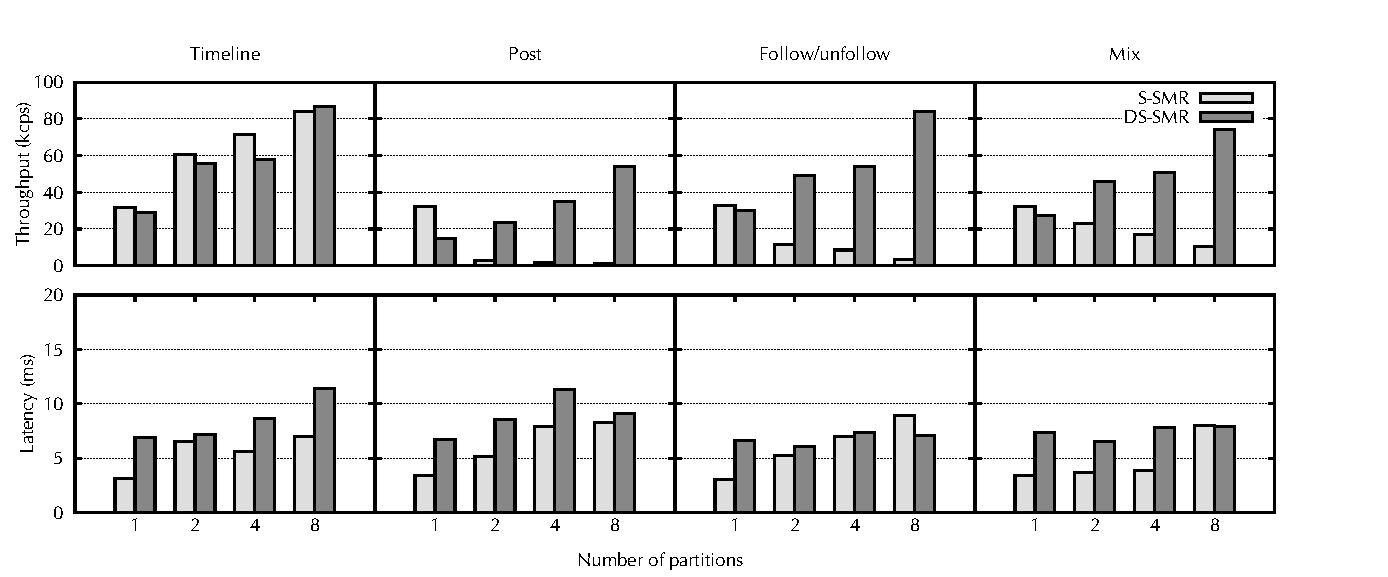
\includegraphics[width=1.08\linewidth]{figures/graphs/strong-locality}
\end{minipage}
\caption{Results of \appname\ running with \ssmr\ and \dssmr{}. Throughput is shown in thousands of commands per second (kcps).}
\label{fig:strongloc}
\end{figure*}

\begin{table*}[htp]
\vspace{10mm}
\caption{Absolute values of \appname\ running \ssmr\ and \dssmr{}.}
\centering
\begin{tabular}{|l|c|c|c|c|c|c|c|c|c|c|c|c|c|c|c|c|} \hline
         & \multicolumn{4}{|c|}{Timeline}  &  \multicolumn{4}{|c|}{Post}   &  \multicolumn{4}{|c|}{Follow/unfollow}  &  \multicolumn{4}{|c|}{Mix}    \\ \hline
         & 1     & 2     & 4     & 8       & 1     & 2     & 4   & 8    & 1     & 2     & 4       & 8           & 1     & 2     & 4     & 8     \\ \hline\hline
         & \multicolumn{16}{|c|}{Throughput (commands per second)} \\ \hline
\ssmr\   & 31757 & 60699 & 71274 & 84065   & 32151 & 2884  & 1894  & 1200  & 32541 & 11476 & 8580    & 3371          & 32151 & 22803 & 16822 & 10657 \\ \hline
\dssmr\  & 28882 & 55925 & 57900 & 86685   & 14874 & 23295 & 35188 & 54250 & 30215 & 48976 & 54025   & 83880         & 27101 & 45686 & 50671 & 74257 \\ \hline\hline
         & \multicolumn{16}{|c|}{\textbf{Throughput rate = \dssmr\ tput / \ssmr\ tput}} \\ \hline
         & \textbf{0.91} & \textbf{0.92}  & \textbf{0.81} & \textbf{1.03}     & \textbf{0.46}   & \textbf{8.08}   & \textbf{18.48}  & \textbf{45.00} & \textbf{0.93} & \textbf{4.27} & \textbf{6.30} & \textbf{24.88} & \textbf{0.84} & \textbf{2.00} & \textbf{3.01} & \textbf{6.97} \\ \hline\hline
         & \multicolumn{16}{|c|}{Latency (milliseconds)} \\ \hline
\ssmr\   & 3.1 & 6.6 & 5.6 & 7.0  & 3.4 & 5.2  & 7.9  & 8.3  & 3.0  & 5.2  & 7.0  & 8.8  & 3.4  & 3.7  & 3.8  & 7.9  \\ \hline
\dssmr\  & 6.9 & 7.1 & 8.6 & 11.4 & 6.7 & 8.6  & 11.3 & 9.1  & 6.6  & 6.1  & 7.4  & 7.0  & 7.3  & 6.5  & 7.8  & 7.9  \\ \hline
\end{tabular}
\label{tbl:results}
\vspace{10mm}
\end{table*}%

\subsection{Environment setup and configuration parameters}
\label{sec:evaluation:setup}

We conducted all experiments on a cluster that had two types of nodes: (a) HP SE1102 nodes, equipped with two Intel Xeon L5420 processors running at 2.5 GHz and with 8 GB of main memory, and (b) Dell SC1435 nodes, equipped with two AMD Opteron 2212 processors running at 2.0 GHz and with 4 GB of main memory. The HP nodes were connected to an HP ProCurve 2920-48G gigabit network switch, and the Dell nodes were connected to another, identical switch. Those switches were interconnected by a 20 Gbps link.
All nodes ran CentOS Linux 7.1 with kernel 3.10 and had the OpenJDK Runtime Environment~8 with the \mbox{64-Bit} Server VM (build 25.45-b02).
%We kept the clocks synchronized using NTP in order to measure latency components involving events in different computers.

For the experiments, we use the following workloads:
Timeline (composed only of getTimeline requests),
Post (only post requests),
Follow/unfollow (50\% of follow requests and 50\% of unfollow), and
Mix (7.5\% post, 3.75\% follow, 3.75\% unfollow, and 85\% getTimeline).

\subsection{Results }
\label{sec:evaluation:strongloc}

% THROUGHPUT

We can see in Figure~\ref{fig:strongloc} and Table~\ref{tbl:results} the results achieved with \appname{}.
%, running with a strong-locality workload.
For the Timeline workload, the throughput with \dssmr\ and \ssmr\ are very similar.
This happens because getTimeline requests are optimized to be single-partition:
all posts in a user's timeline are stored along with the User object.
%Every getTimeline requests accesses a single User object (of the user whose timeline is being requested).
This is the ideal workload for \ssmr{}.
In \dssmr{}, the partitioning does not change, and consulting the oracle becomes unnecessary thanks to the local cache at each client.
This happens because there are no other commands in the Timeline workload.

In the Post workload, every command accesses up to all partitions in the system, which is the worst case for \ssmr{}: the more partitions are involved in the execution of a command, the worst is the system's performance.
We can see that the throughput of \ssmr\ decreases significantly as the number of partitions increases.
For \dssmr{}, we can see that the system throughput scales with the number of partitions.
This happens because User objects that are accessed together, but which are in different partitions, are moved to the same partition based on the interests of the users.
In the case of post command on 2 partitions, the number of move commands started ~3kcps, over 23kps of throughput, then reduced to less than 0.1kcps over time.\fxnote[draft]{Add ratio of move command}
As the execution proceeds, this leads to a lower rate of multi-partition commands, which allows throughput to scale.
As a result the throughput improvement of \dssmr{} with respect to \ssmr\ increases over time.
With eight partitions, \dssmr{} sports a performance that is 45 times that of \ssmr!

With the Follow/unfollow workload, the system performs in a similar way to that observed with the Post workload.
The difference is that each follow or unfollow request accesses only two User objects, whereas every post request may affect an unbounded number of users.
For this reason, each follow/unfollow command is executed at most by two partitions in \ssmr{}.
In \dssmr{}, a single move command is enough to have all User objects affected by such a command in the same partition.
For this reason, both replication techniques have better throughput under the Follow/unfollow workload than with Post.
As with the Post workload, \dssmr{}'s advantage over \ssmr\ increases with the number of partitions, reaching up to almost 25 times with eight partitions.

We approximate a realistic distribution of commands with the Mix workload.
With such a workload, \ssmr\ does not perform as bad as in the Post or Follow/unfollow workloads, but the system throughput still decreases as partitions are added.
As with the other workloads, \dssmr\ scaled under the Mix workload.
With eight partitions, it reached 74~kcps (thousands of commands per second), fairly close to the ideal case (the Timeline workload), where \dssmr\ reached 86~kcps.
Under the Mix workload, \ssmr\ had less than 33~kcps in the best case (one partition) and around 10~kcps with eight partitions.
In the configuration with eight partitions, \dssmr\ reaches almost seven times \ssmr's throughput.

Latency values with \dssmr\ are higher than with \ssmr{}.
This was expected for two reasons. First, there is an extra group of servers (the oracle) to communicate with.
Second, executing a command often means moving all accessed objects to the same partition.
Taking this into account, we consider the (often slight) increase in latency observed with \dssmr\ a low price to pay for the significant increase in throughput and the scalability that \dssmr\ brought to the system; with \ssmr{}, the system did not scale with multi-partition commands.



%\subsection{Results for weak locality}
%\label{sec:evaluation:weakloc}
%!TEX root =  main.tex
\section{Related work}
\label{sec:rw}

State machine replication~\cite{Kapritsos:2012um, kotla2004htbft, Lam78, santos2013htsmr, Sch90} provides strong consistency guarantees, which come from total order and deterministic execution of commands.
%Deterministic execution is usually ensured by having every replica execute commands sequentially.
Since consistent ordering is fundamental for SMR, some authors proposed to optimize the ordering and propagation of commands.
% (i.e., the atomic broadcast layer of the system).
For instance, \cite{kapritsos2010scalable} proposes to divide the ordering of commands between different clusters: each cluster orders only some requests, and then forwards the partial order to every server replica, which then merges the partial orders deterministically into a single total order that is consistent across the system.
In~\cite{biely2012spaxos}, Paxos~\cite{Lamport:1998ea} is used to order commands, but it is implemented in a way that avoids overloading the leader process, which would turn it into a bottleneck.

Multi-threaded execution is a potential source of non-determinism, depending on how threads are scheduled to be executed in the operating system.
Some works attempted to circumvent this problems and come up with a multi-threaded, yet deterministic implementation of SMR.
In \cite{santos2013htsmr}, the authors propose to parallelize the receipt and dispatching of commands, while executing commands sequentially.
In \cite{kotla2004htbft}, application semantics is used to determine which commands can be executed concurrently and still produce a deterministic outcome (e.g., read-only commands).
In \cite{Kapritsos:2012um}, commands are tentatively executed in parallel.
After the parallel execution, replicas verify whether they reached a consistent state; if not, commands are rolled back and re-executed sequentially.

Many database replication schemes aim at achieving high throughput by relaxing consistency, that is, they do not ensure linearizability.
In deferred-update replication \cite{chundi96dur, kobus2013hybrid, sciascia2012sdur, SousaOMP01}, replicas commit read-only transactions immediately, not always synchronizing with each other.
Although this indeed improves performance, it allows non-linearizable executions.
Database systems usually ensure serializability \cite{BHG87} or snapshot isolation \cite{LinKJPA09}, which do not take into account real-time precedence of different commands among different clients. 
For some applications, these consistency levels may be enough, allowing the system to scale better, but services that require linearizability cannot be implemented with such techniques.

Efforts to make linearizable systems scalable have been made in the past~\cite{bezerra2014ssmr, corbett2013spanner, Glendenning2011, hoang2016, Marandi11}.
In \cite{Glendenning2011}, the authors propose a scalable key-value store based on DHTs, ensuring linearizability, but only for requests that access the same key. 
In \cite{Marandi11}, variant of SMR is proposed in which data items are partitioned but commands have to be totally ordered.
Spanner~\cite{corbett2013spanner} uses a separate Paxos group per partition and, to ensure strong consistency across partitions, clocks are assumed to be synchronized.
Although the authors say that Spanner works well with GPS and atomic clocks, if clocks become out of synch beyond tolerated bounds, correctness is not guaranteed.
\ssmr{}~\cite{bezerra2014ssmr} ensures consistency across partitions without any assumption about clock synchronization, but relies on a static partitioning of the state.
\dssmr{}~\cite{hoang2016} extends \ssmr\ by allowing state variables to migrate across partitions in order to reduce multi-partition commands.
However, \dssmr{} implements repartitioning in a very simple way that does not perform very well in scenarios with weak locality.
\dynastar\ improves on \dssmr\ by employing well-known graph partitioning techniques to decide where each variable should be.
Moreover, \dynastar\ dillutes the cost of repartitioning by moving variables on-demand, that is, only when they are accessed by some command.

Graph partitioning is an interesting problem with many proposed solutions~\cite{Abou-Rjeili:2006,kernighan1970efficient,hendrickson2000graph}.
In this work, we do not introduce a new graph partitioning solution, but instead we use a well-known one (METIS~\cite{Abou-Rjeili:2006}) to partition the state of a service implemented with state machine replication.
Similarly to \dynastar{}, Schism~\cite{curino2010sch} and Clay~\cite{SerafiniTEPAS16} also use graph-based partitioning to decide where to place data items in a transactional database.
In either case, not much detail is given about how to handle repartitioning dynamically without violating consistency.
Sword~\cite{quamar2013sword} is another graph-based dynamic repartitioning technique.
It uses a hypergraph partitioning algorithm to distribute rows of tables in a relational database across database shards.
Sword does not ensure linearizability and it is not clear how it implements repartitions without violating consistency.
E-Store~\cite{taft2014est} is yet another repartitioning proposal for transactional databases.
It repartitions data according to access patterns from the workload.
It strives to minimize the number of multi-partition accesses and is able to redistribute data items among partitions during execution.
E-Store assumes that all non-replicated tables form a tree-schema based on foreign key relationships.
This has the drawback of ruling out graph-structured schemas and \mbox{$m$-$n$} relationships.
\dynastar\ is a more general approach that works with any kind of relationship between data items, while also ensuring linearizability.

Some replication schemes are ``dynamic'' in that they allow the membership to be reconfigured during execution (e.g., \cite{birman2010dsr,dustdar2007soc,guessoum2003dar}).
For instance, a multicast layer based on Paxos can be reconfigured by adding or removing acceptors. 
These systems are dynamic in a way that is orthogonal to what \dynastar\ proposes.
%\dynastar\ consists of allowing the \emph{state partitioning}, that is, which state variables belong to which partition, to change dynamically.
%The greatest challenge that is addressed by \dynastar\ is how to provide such a solution, with a dynamic partitioning oracle, while ensuring a very strong level of consistency (linearizability), as variables are created, deleted, and moved across partitions, based on the access patterns of the workload.


\section{Conclusion}
\label{sec:conclusion}

This work introduces S-SMR, a scalable variant of the well-known state-machine replication technique. 
S-SMR differs from previous related works in that it allows throughput to scale with the number of partitions without weakening consistency. 
To evaluate S-SMR, we developed the Eyrie library and implemented Volery, a Zookeeper clone, with Eyrie.
Our experiments demonstrate that in deployments with 8 partitions (the largest configuration we can deploy in our infrastructure) and under certain workloads, throughput experienced an 8-time improvement, resulting in ideal scalability.
Moreover, Volery's throughput proved to be significantly higher than Zookeeper's.

\bibliographystyle{abbrv}
\bibliography{references}

%!TEX root =  main.tex
\clearpage
\subsection{Correctness}
\label{sec:correctness}

In this section, we argue that \dynastar is safe (i.e., it ensures linearizability) and live (i.e., it ensures termination).

To prove that \dynastar ensures linearizability, we must show that for any execution $\sigma$ of the system, there is a total order $\pi$ on client commands that 
(i)~respects the semantics of the commands, as defined in their sequential specifications, and 
(ii)~respects the real-time precedence of commands~(Section~\ref{sec:correctcrit}).
%
Let $\pi$ be a total order of operations in $\sigma$ that respects $<$, the order atomic multicast induces on commands.

To argue that $\pi$ respects the semantics of  commands, let $C_i$ be the $i$-th command in $\pi$ and $p$ a process in partition $\ppm_p$ that executes $C_i$.
%Let $C_i$ be the $i$-th command in $\pi$ and $p$ a process in partition $\ppm_p$ that executes $C_i$.
We claim that when $p$ executes $C_i$, it has updated values of variables in $vars(C_i)$, the variables accessed by $C_i$.
We proof the claim by induction on $i$.
The base step trivially holds from the fact that variables are initialized correctly.
Let $v \in vars(C_i)$, $C_v$ be the last client command before $C_i$ in $\pi$ that accesses $v$, and $q$ a process in $\ppm_q$ that executes $C_v$.
From the inductive hypothesis, $q$ has an updated value of $v$ when it executes $C_v$.
There are two cases to consider:
(a)~$p = q$. In this case, $p$ obviously has an updated value of $v$ when it executes $C_i$ since no other command accesses $v$ between $C_v$ and $C_i$.
(b)~$p \neq q$. 
Since processes in the same partition execute the same commands, it must be that $\ppm_p \neq \ppm_q$.
From the algorithm, when $q$ executes $C_v$, $v \in \ppm_q$ and when $p$ executes $C_i$, $v \in \ppm_p$.
Thus, $q$ executed a command to move $v$ to another partition after executing $C_v$ and $p$ executed a command to move $v$ to $\ppm_p$ before executing $C_i$.
Since there is no command that accesses $v$ between $C_v$ and $C_i$ in $\pi$, $q$ has an updated $v$ when it executes $C_v$ (from inductive hypothesis), and $p$ receives the value of $v$ at $q$, it follows that $p$ has an updated $v$ when it executes $C_i$.

% DISCLAIMER: in the proof below, I assumed a single process per partition. While I'm pretty sure it works for multiple processes per partition, in some future refinement this should be added to the proof. Also see related picture showing cases (a) and (b) below. Perhaps we should include such a picture too in a future version.
%
We now argue that there is a total order $\pi$ that respects the real-time precedence of commands in $\sigma$.
Assume $C_i$ ends before $C_j$ starts, or more precisely, the time $C_i$ ends at a client is smaller than the time $C_j$ starts at a client, $tec(C_i) < tsc(C_j)$.
Since the time $C_i$ ends at the server from which the client receives the response for $C_i$ is smaller than the time $C_i$ ends at the client, $tes(C_i) < tec(C_i)$, and the time $C_j$ starts at the client is smaller than the time $C_j$ starts at the first server, $tsc(C_j) < tss(C_j)$, we conclude that $tes(C_i) < tss(C_j)$.

We must show that either $C_i < C_j$; or neither $C_i < C_j$ nor $C_j < C_i$.
For a contradiction, assume that $C_j < ... < Z_k < ... < C_i$, where $Z_k$ is a client or a move command.
Let $Z_k$ be delivered by partition $\ppm_k$.
There are two cases: 
\begin{enumerate}
\item[(a)] $Z_{k+1}$ is a client command delivered by partition $\ppm_k$.
In this case, since $Z_{k+1}$ only starts after $Z_k$ at a server, it follows that $tes(Z_k) < tss(Z_{k+1})$.
\item[(b)] $Z_{k+1}$ is a move command that involves $\ppm_k$ as source and $\ppm_{k+1}$ as destination.
At $\ppm_k$, $tes(Z_k) < tss(Z_{k+1})$ since the move is only executed after $Z_k$.
Since servers in $\ppm_k$ must send one or more variables to servers in $\ppm_{k+1}$, it must be that $tss(Z_{k+1}) < tes(Z_{k+1})$.
Thus, it follows that $tes(Z_{k+1}) < tss(Z_{k+2})$.
\end{enumerate}
From the two cases above, we conclude that $tes(C_j) < tss(C_i)$, a contradiction.
Therefore, either $C_i < C_j$ and from the definition of $\pi$, $C_i$ precedes $C_j$ or neither $C_i < C_j$ nor $C_j < C_i$, and there is a total order in which $C_i$ precedes $C_j$.
%\begin{figure}
%\centering
%\includegraphics[width=1.2\linewidth,angle=-90]{figures/IMG_7203.JPG}
%\caption{Two cases in proof.}
%\end{figure}

For termination, we argue that every correct client eventually receives a reply different than $retry$ for every command $C$ that it issues.
This assumes that every partition (including the oracle partition) is always operational, despite the failure of some servers in the partition.
For a contradiction, assume that some client submits a command $C$ that always returns $retry$.
Therefore, from the algorithm, whenever $C$ is delivered at a partition, the partition does not contain all the variables needed by $C$.
As a consequence, the client eventually falls back to \ssmr\ and multicasts $C$ to all partitions and $C$ is executed as a multi-partition command, which is guaranteed to succeed, a contradiction that concludes our argument.




\end{document}
